\documentclass[Orator]{subfiles}
\begin{document}


\section{Our Approach}

\subsection{The inspiration}

\subsection{Input}
\indent Since we want want minimize the effects of a possible bias in our data, it makes sense to use the Gaussian white noise signal as an input. But why? \newline
\indent \textbf{White noise:} random signal having equal intensity at different frequencies 
FINISH THIS!
\begin{figure}[h]
    \centering
    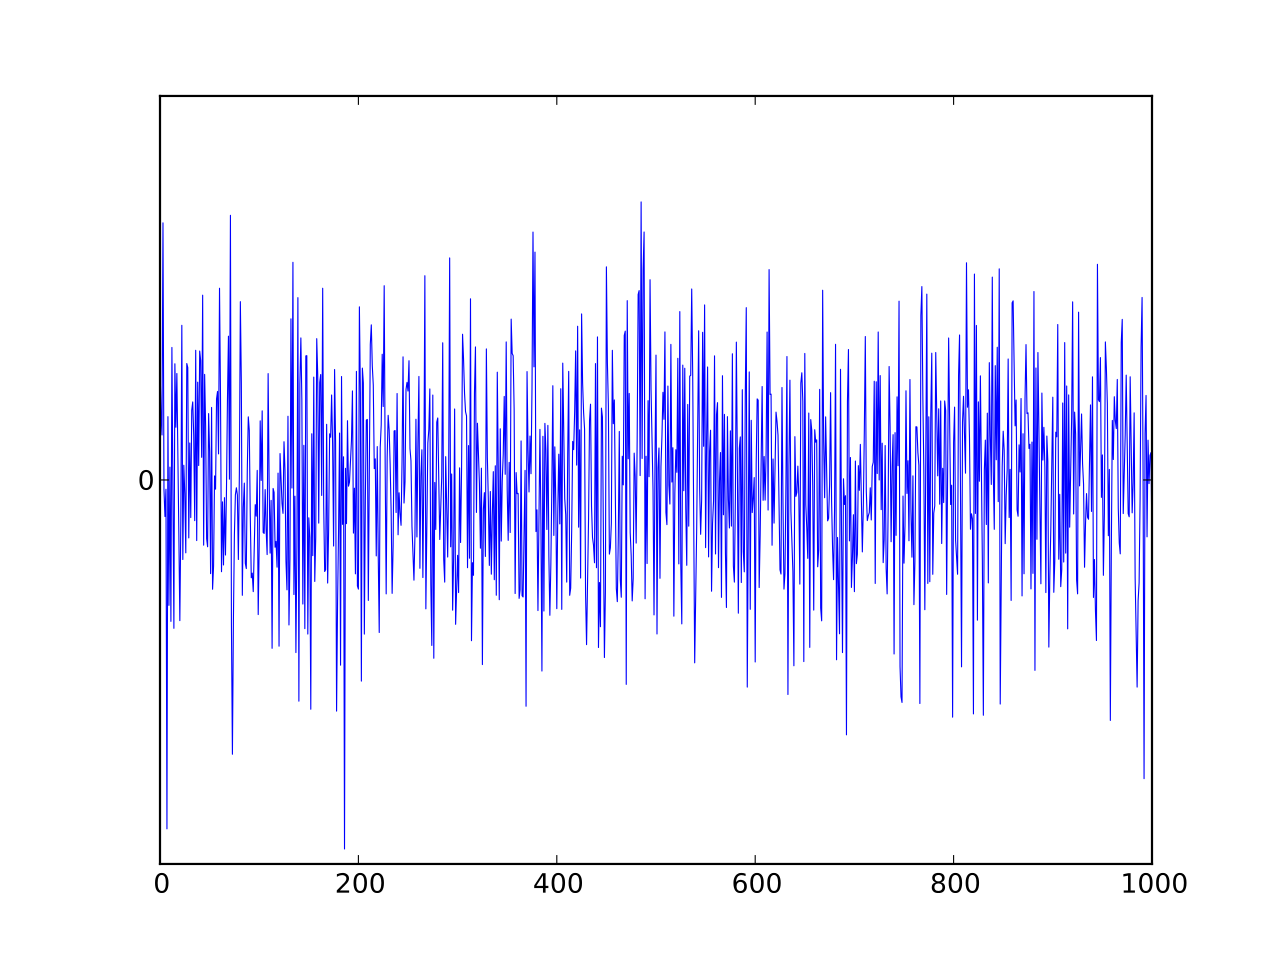
\includegraphics[width=300 pt]{Pictures/Ana/White_noise.svg.png}
    \caption{The waveform of a Gaussian white noise signal plotted on a graph \cite{https://en.wikipedia.org/wiki/White_noise#/media/File:White_noise.svg}.}
    \label{fig:HH circuit}
\end{figure}
\subsection{Neuronal Motif}



\end{document}